\chapter{Background}

For planning purposes, it is important to know the maximum voltage that can be
transferred with transmission lines to meet the anticipated load demand. It is also important to know the levels of power through various transmission lines under certain contingency outage conditions to maintain the continuity of service. Knowledge of power flows and voltage levels under normal operating conditions are necessary in order to determine fault currents and the ensuing consequences on the transient stability of the system. \\
Determining power flow requires measurements of some power system conditions; utilities measure a combination of quantities such as voltage magnitude \gls{V}, real power \gls{P} and reactive power \gls{Q} \cite{eps}.

\section{Description of a power system}
%https://www.generatorsource.com/Articles/Generator-Info/High-Medium-and-Low-Voltage-Differences.aspx
In the traditional power system, electricity is produced in large, centralised power plants. The electricity is then transferred to the loads using the transmission and distribution networks. High and extra-high voltages are associated with supply transmission from the power plant. The reason for transmitting power at high and extra-high voltage levels is to increase efficiency. The lower current accompanying the high voltage transmission allows for the use of thinner lighter-weight cables. This reduces the cost in the tower and electrical line construction. High and extra-high voltages refer to voltage magnitudes between $35 kV \leq V < 220 kV$ for the high voltage and $V \geq 220 kV$ for the extra high voltage. \\
Large industrial complexes and factories that require a substantial amount of power often utilise medium supply voltages. The high voltage coming from the power plant is sent to the primary substation, this can supply step-down power to secondary substations or to single buildings. Secondary substations can have transformers to further step down the power, and they are generally located in areas that can serve one or more buildings. Medium voltages refer to voltage magnitude $1 kV \leq V < 35 kV$. \\
Then the medium supply power is step down again to a low voltage and sent to the domestic household or home appliances power supply. Low voltages refer to voltage magnitude between $V < 1 kV$. \\
\begin{figure}[h]
\centering
    % 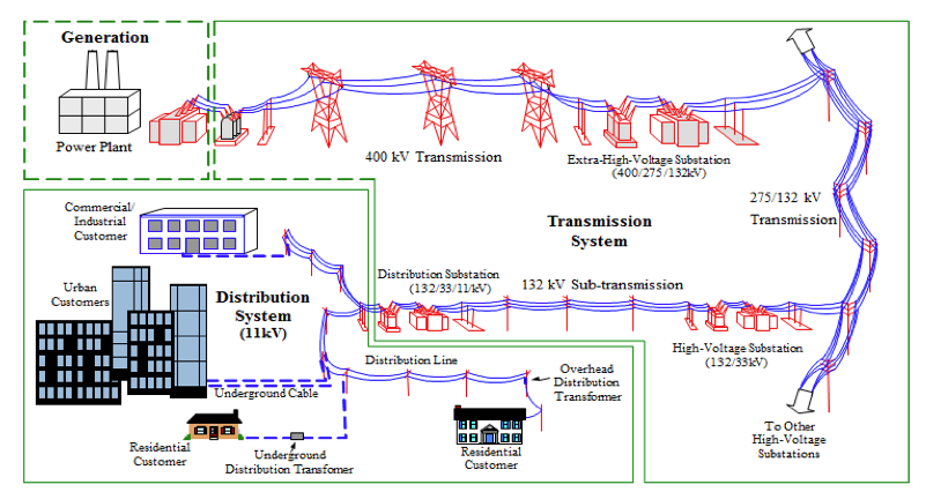
\includegraphics[width=.9\linewidth]{images/DN/HighMediumLowV.png}
    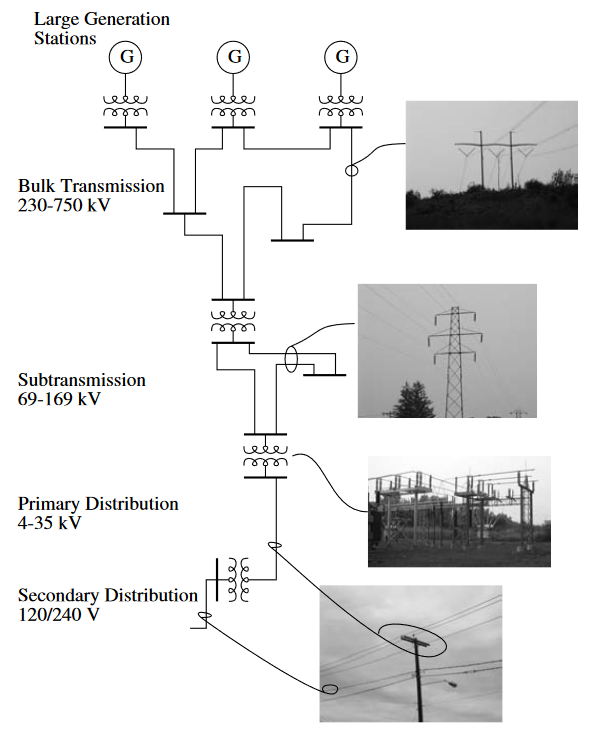
\includegraphics[width=.5\linewidth]{images/DN/DN.PNG}
\caption[Power network distribution]{Power network distribution \cite{EPD}\\}
% \label{fig:gym_anm_net}
\end{figure}


\noindent A power system is usually made up of the following main elements:
\begin{itemize}
    \item Load buses where \gls{P} and \gls{Q} are specified.
    \item Generator buses where the voltage magnitude \gls{V} and the power \gls{P} are specified.
    \item A primary bus, an "infinite" bus, where the magnitude voltage \gls{V} is specified (normally 1 \gls{pu}) and its phase angle \gls{Vangle} is assumed to be zero as a reference angle. At this bus, both \gls{P} and \gls{Q} can be what is needed to keep the network stable. \cite{eps}
\end{itemize}

